\header{
    \section{Y'a quatre marins} \label{y-a-quatre-marins}
    %
    \insertComment{Chanson de Hugues Aufray.}{}
}

\enluminure{3}{\href{https://www.youtube.com/watch?v=6ewLUKHZ_b8&list=PL_Qtm8SvoiAJNsalyDwb5zsb4WxM_TGzL&index=12}{Y}}~\\
$\left.\begin{tabular}{l}
\hspace{-0.4cm}
\textsc{'a quatre} marins sur la mer
\\
\hspace{-0.4cm}
Loin de leur amitié
\\
\hspace{-0.4cm}
Loin de leur amitié
\end{tabular}\right\rbrace$ bis\\\\
\bisquadruplespace{Quand ils viendront à terre}
{Géflalala lalalire}
{Nous les ferons danser}
{Géflala laridé}
\bistriplespace{Mais la vague est profonde}
{Et le vent déchaîné}
{Et le vent déchaîné}
\bisquadruplespace{De l'horizon qui gronde}
{Monte une houle sans pitié}
{C'est la misère du monde}
{Qui cogne au chalutier}
\bistriplespace{Y'a bien de la souffrance}
{Pour les gens de la mer}
{Pour les gens de la mer}
\bisquadruplespace{Le coeur plein de vaillance}
{Durs au labeur solitaire}
{Aux croisées de l'absence}
{Ils chantent leur calvaire}
\bistriplespace{Y'a quatre marins-pêcheurs}
{Aux portes de l'enfer}
{Aux portes de l'enfer}
\\\bisquadruplespace{Mais le canot des sauv'teurs}
{A entendu leurs prières}
{Bravant le diable et la peur}
{Il les ramène à terre}
\\\bistriplespace{Y'a quatre marins sur la terre}
{Près de leurs bien-aimées}
{Près de leurs bien-aimées}
\bisquadruplespace{Demain dès l'aube claire ~~~~~}
{Géflalala lalalire}
{Ils reprendront la mer}
{Géflala laridé}
\bisdouble{Y'a quatre marins sur la mer}
{Loin de leur amitié}
\bigskip
\bigskip
\bigskip
\begin{center}
\centering
    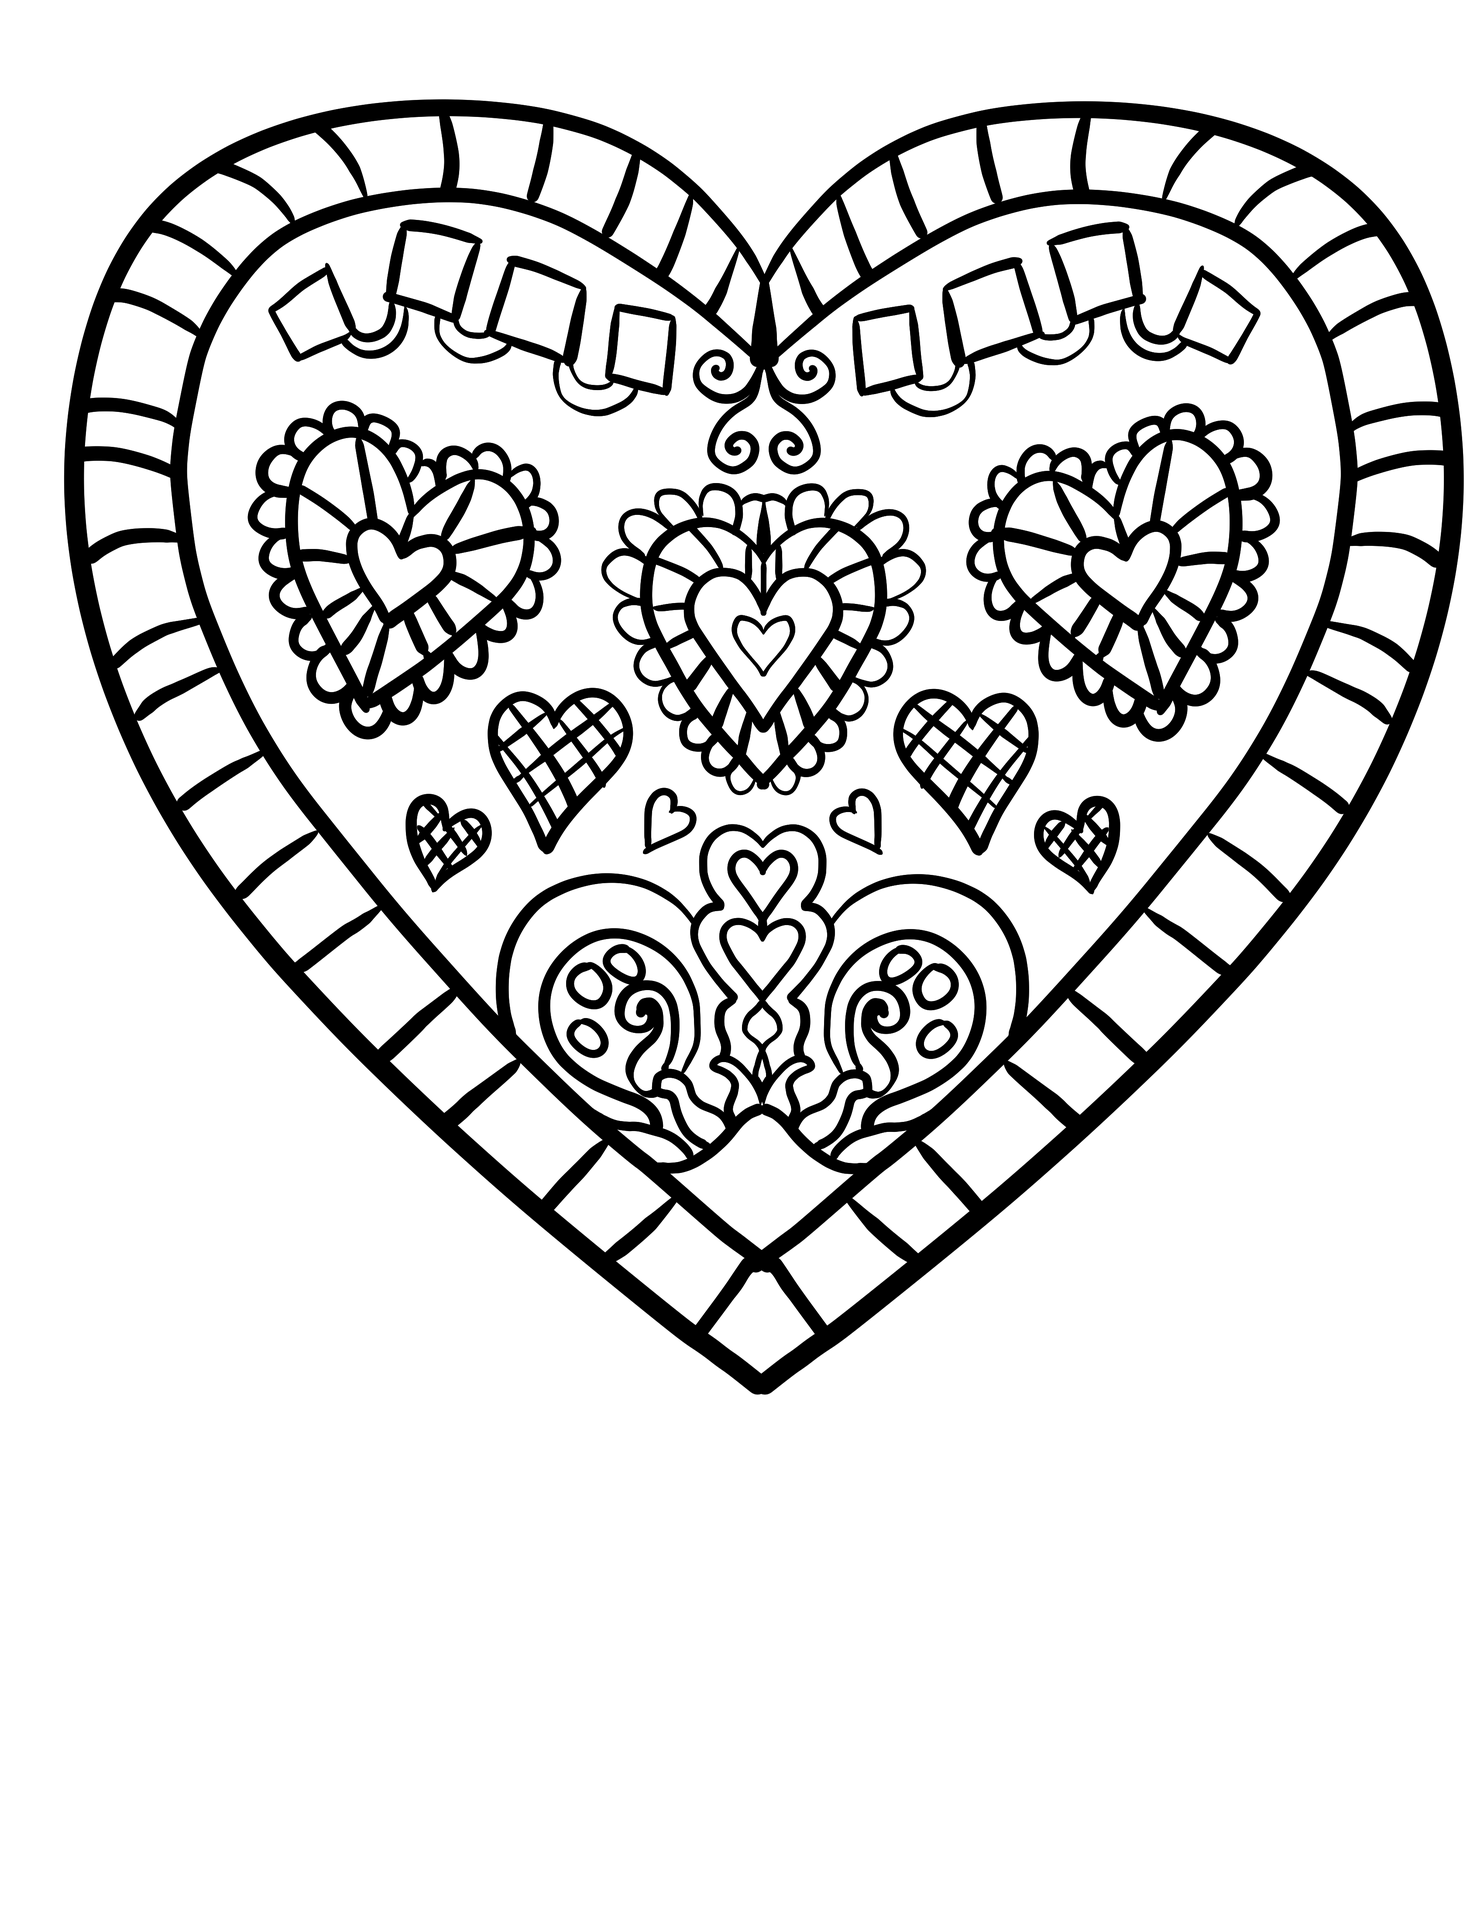
\includegraphics[width=0.7\textwidth]{images/brev74.png}
 \end{center}

\breakpage